\documentclass[a4paper,12pt]{article}

\usepackage[spanish]{babel}
\usepackage[utf8]{inputenc}
\usepackage[T1]{fontenc}
\usepackage[utf8]{inputenc}
\usepackage{makeidx}
\usepackage{graphicx}
\usepackage{lmodern}
\usepackage{kpfonts}
\usepackage[left=2cm,right=2cm,top=2cm,bottom=2cm]{geometry}
\usepackage{amsmath,amsfonts,amssymb}
\usepackage{hyperref}
\hypersetup{
    colorlinks=true,
    linkcolor=cyan,
    filecolor=magenta,      
    urlcolor=blue,
    pdftitle={titulo},
    pdfpagemode=FullScreen,
    }
\urlstyle{same}

\title{Asignación 1}

\begin{document}

\begin{center}
\par 
\includegraphics[scale=1]{USB} \par
Universidad Simon Bolivar \\ Curso: CI4325 / Interfaces con el Usuario \\ Trimestre: Enero-Marzo, 2024 \\ Profesor: Franco Gabriel Nori Gonzalez \\ Estudiante: Junior Miguel Lara Torres - Carnet: 17-10303 \\
\end{center}

\begin{center}
Asignación 1 (5\%)
\end{center}

\begin{itemize}

\item Busque y seleccione una imagen (puede ser una serie, película o una fotografía) que refleje cada uno de los conceptos:

\begin{itemize}
\item Icono, símbolo y signo. (1,5 puntos).
\end{itemize}

\begin{center}
\par 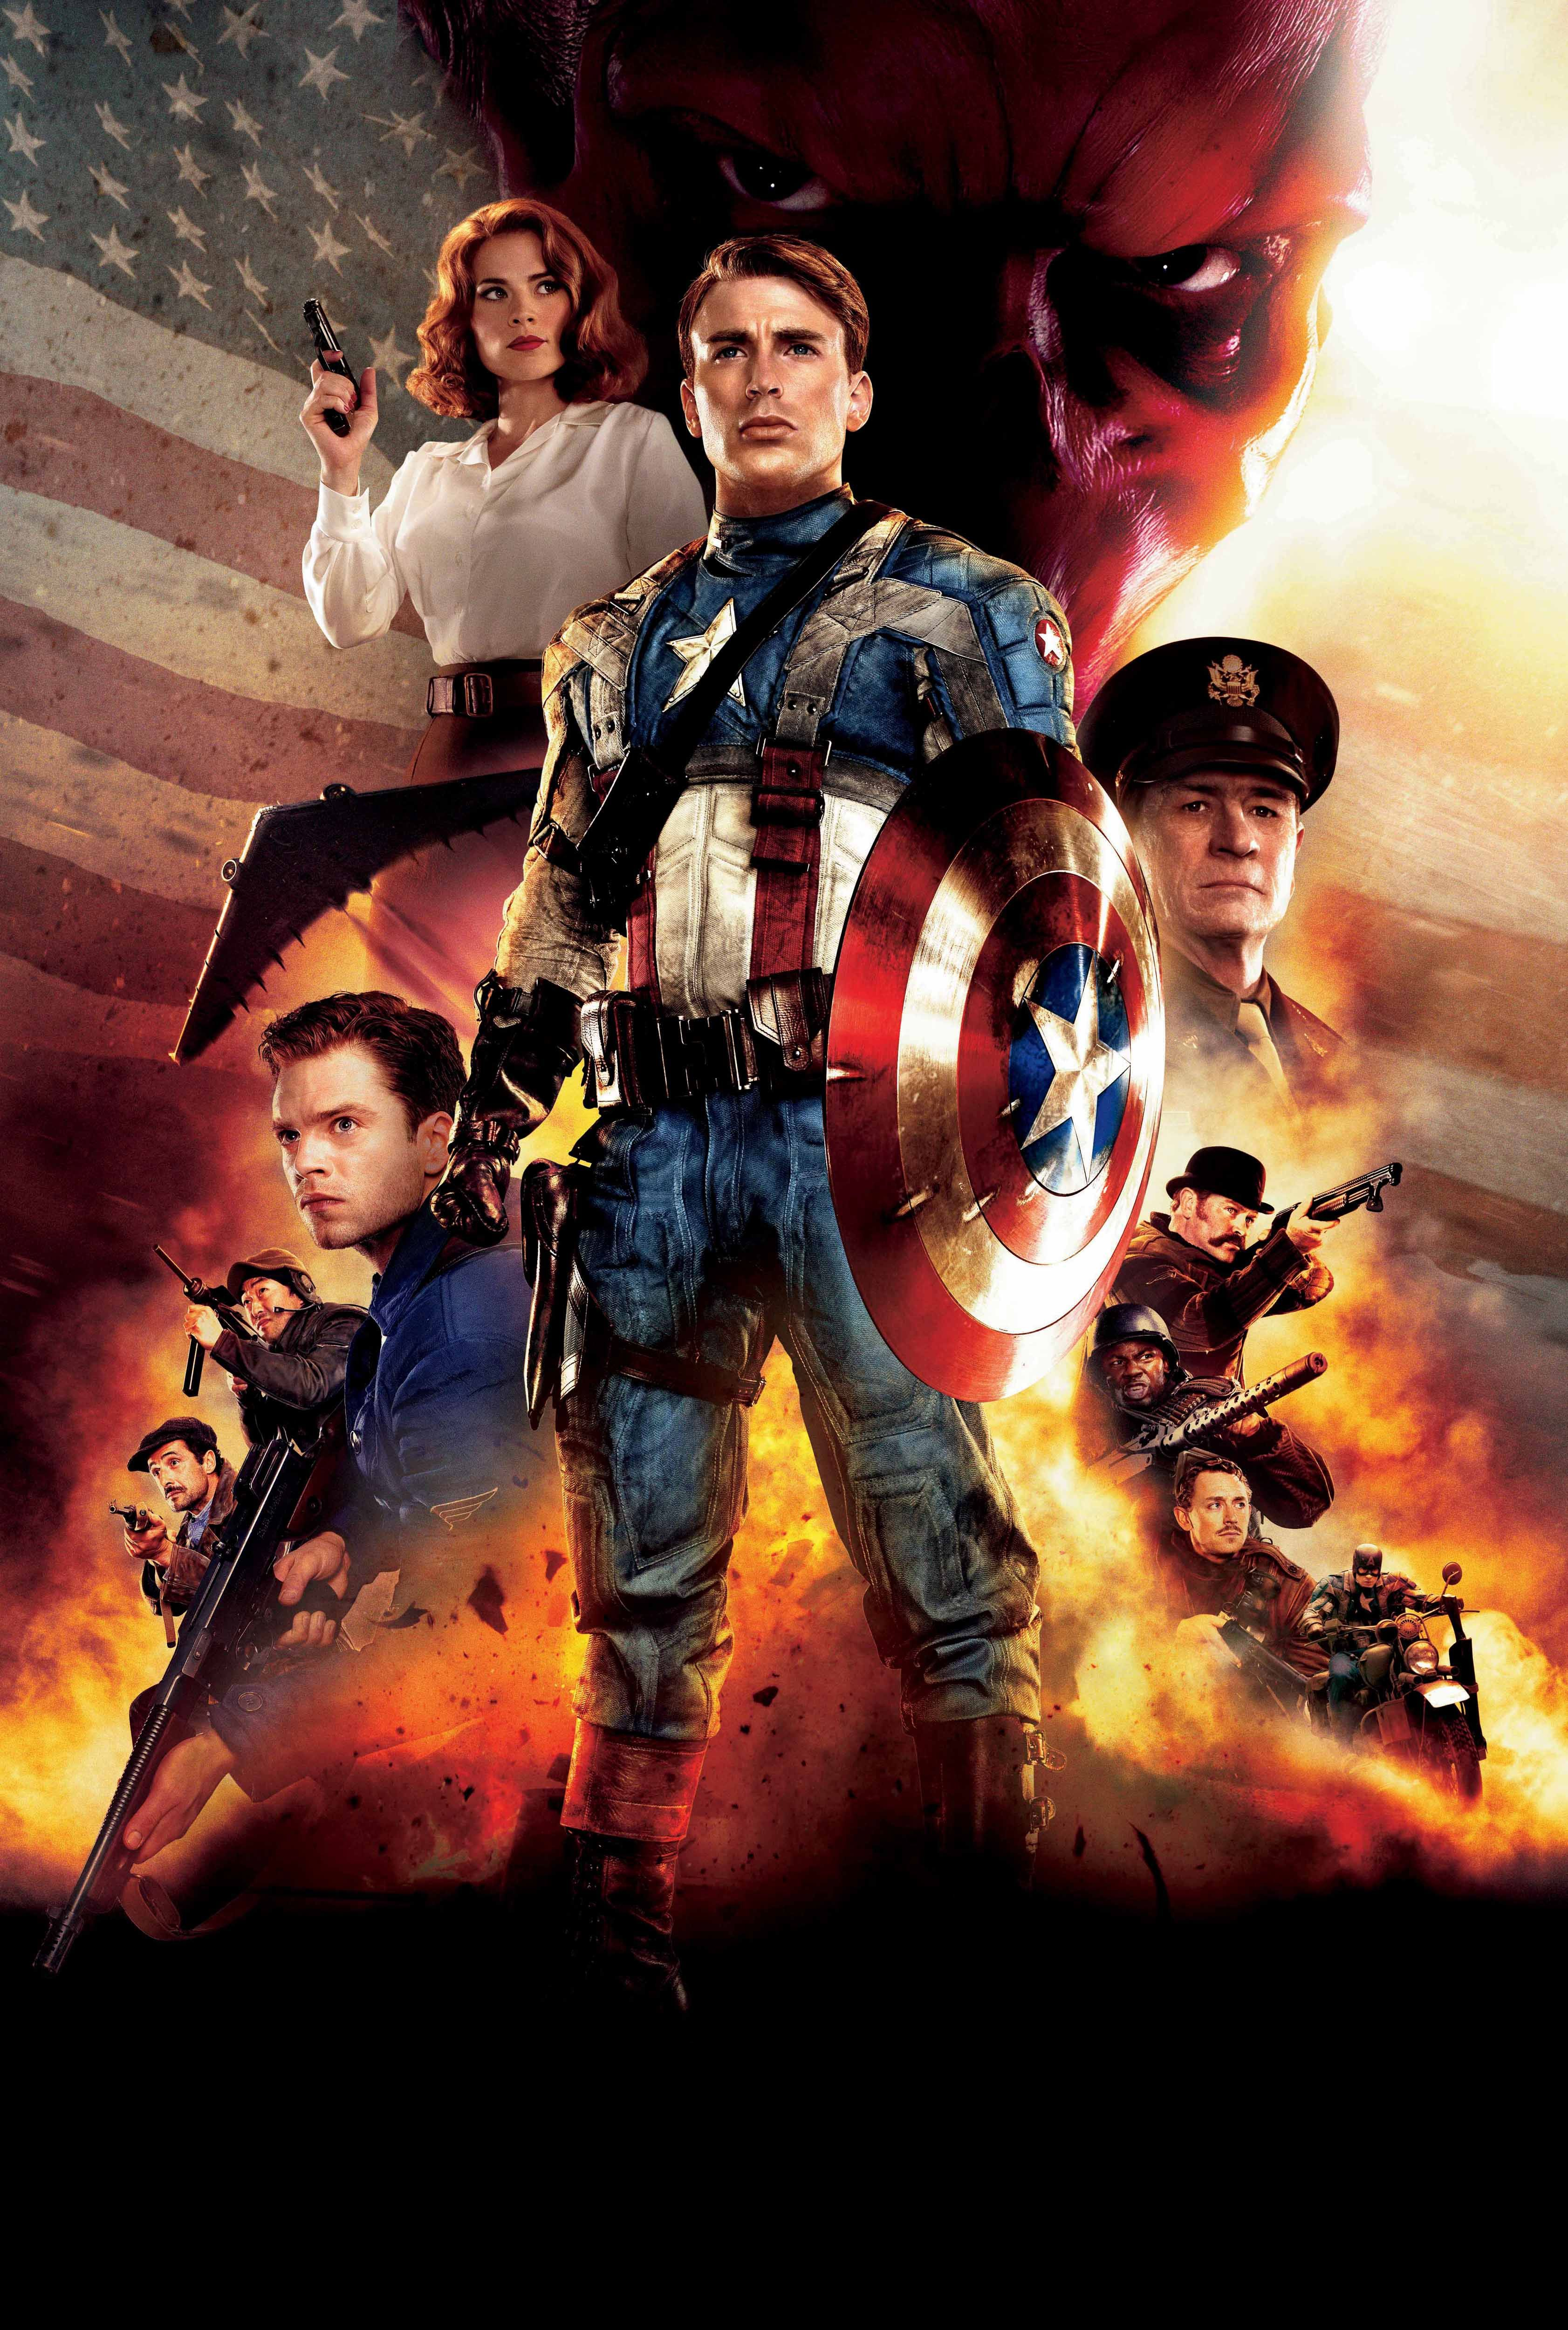
\includegraphics[scale=0.07]{capitanamerica.jpg} \par
\begin{itemize}
\item Icono: Chris Evans (Actor)
\item Simbolo: Luchar por su país y la libertad (Personaje Cap. América)
\item Signo: Estrella (Dibujada en el centro del escudo)
\end{itemize}
\end{center}

\item Enumere 3 ideas propias de un producto que usted diseñaría. Para cada producto enumere una hipótesis principal (del problema a resolver). (1,5 puntos).

\begin{itemize}
\item La mayoria de los Cyber mantienen su sistema de permisos tradicionales para instalar nuevos apps/juegos en las computadoras cuando un cliente lo desea. El metodo mas tradicional es que el dueño o encargado viene personalmente a colocar la clave desbloquear la proteccion contra apps maliciosas o de dudosa procedencia. Se propone crear un software que tenga en red a todas las computadoras incluyendo la del administrador, cuando un cliente quiera instalar alguna nueva app o juego en general este software manda un aviso en tiempo real a la maquina principal donde el gerente/persona a cargo debe rebocar o admitir dicha solicitud.
\item Las tiendas convencionales tienden a vender huevos en cartones que son desechables, el cual representa un despirfarro de dinero y recursos. Se propone que la tienda venda un envase comodo de vidrio flexible que sirva con la funcionalidad de recargarce con nuevos huevos. Asi mismo la tienda dede tener un multienvase del mismo materia tal que sea recargaba en masa por la compañia proveedora. 
\item En situaciones ameritamos hidratarnos, ya sea por simple querer, deportes o cualquier otra razon, la disposicion de agua se hace difícil en ocasiones. Se propone crear un filtro de agua compacto y fácil de transportar, así las personas podrán purificar el agua de fuentes naturales durante sus viajes o en momentos de emergencia, evitando enfermedades transmitidas por el agua contaminada.
\end{itemize}

\item Elabore un “pitch” en video (máximo 1 minuto) de alguno de los productos presentados (el de su preferencia) en el que presente la idea y la hipótesis del problema a resolver. (2 puntos).

\end{itemize}

\end{document}
